\chapter{Proposed algorithm and real world applications}
\label{chapter:algorithm}

In Chapter 

\section{From experimental results to solution}
\label{sec:proposed algorithm}

\subsection{Optimal number of communities}
\label{subsec:optimal beta}

\subsection{Hierarchical topology}
\label{subsec:hierarchical}

More complex small world and scale free graphs allow us to model more realistically human and computer networks, but they still have certain fallacies.
Scale free networks simulate the popularity effect through its peripheral attachment mechanism, making certain nodes more probable to have higher degree with respect to others.
However scale free network do not enable us to simulate high clustering around the whole network, clustering is generated only at the \textit{central} nodes, the ones with high degree.
On the other hand, small world graphs have high clustering property, intrinsic in it's algorithm definition, but the degree of each node is the same.

We find both approaches lacklustre, for within human networks as well as human-made we can observe the difference of link quantity between different nodes.
The peripheral attachment property seems present in most systems studied for the purpose of this thesis.
Likewise the clustering is also a real phenomenon, that can be observed easily in systems studied, for example the different branches of financial markets form loosely connected communities, divided whether by the object of their trading or by the place of their operation.

In an attempt to model competitive systems more closely we have decided to merge two different characteristics from small world and scale free graphs into a hybrid networks, that we call hierarchical network.
Single communities are formed by using the Barabasi-Albert algorithm in order to obtain the peripheral attachment property.
After $C$ communities have been generated they are united in a larger community and a second step of the Watts-Strogatz algorithm is executed to create a short average length between different communities.
If a high enough degree parameter is given to the Barabasi-Albert algorithm we can obtain locally high clustering, while maintaining the short average length between nodes with Watts-Strogatz application to the entire network.

\begin{figure}[h]
\centering
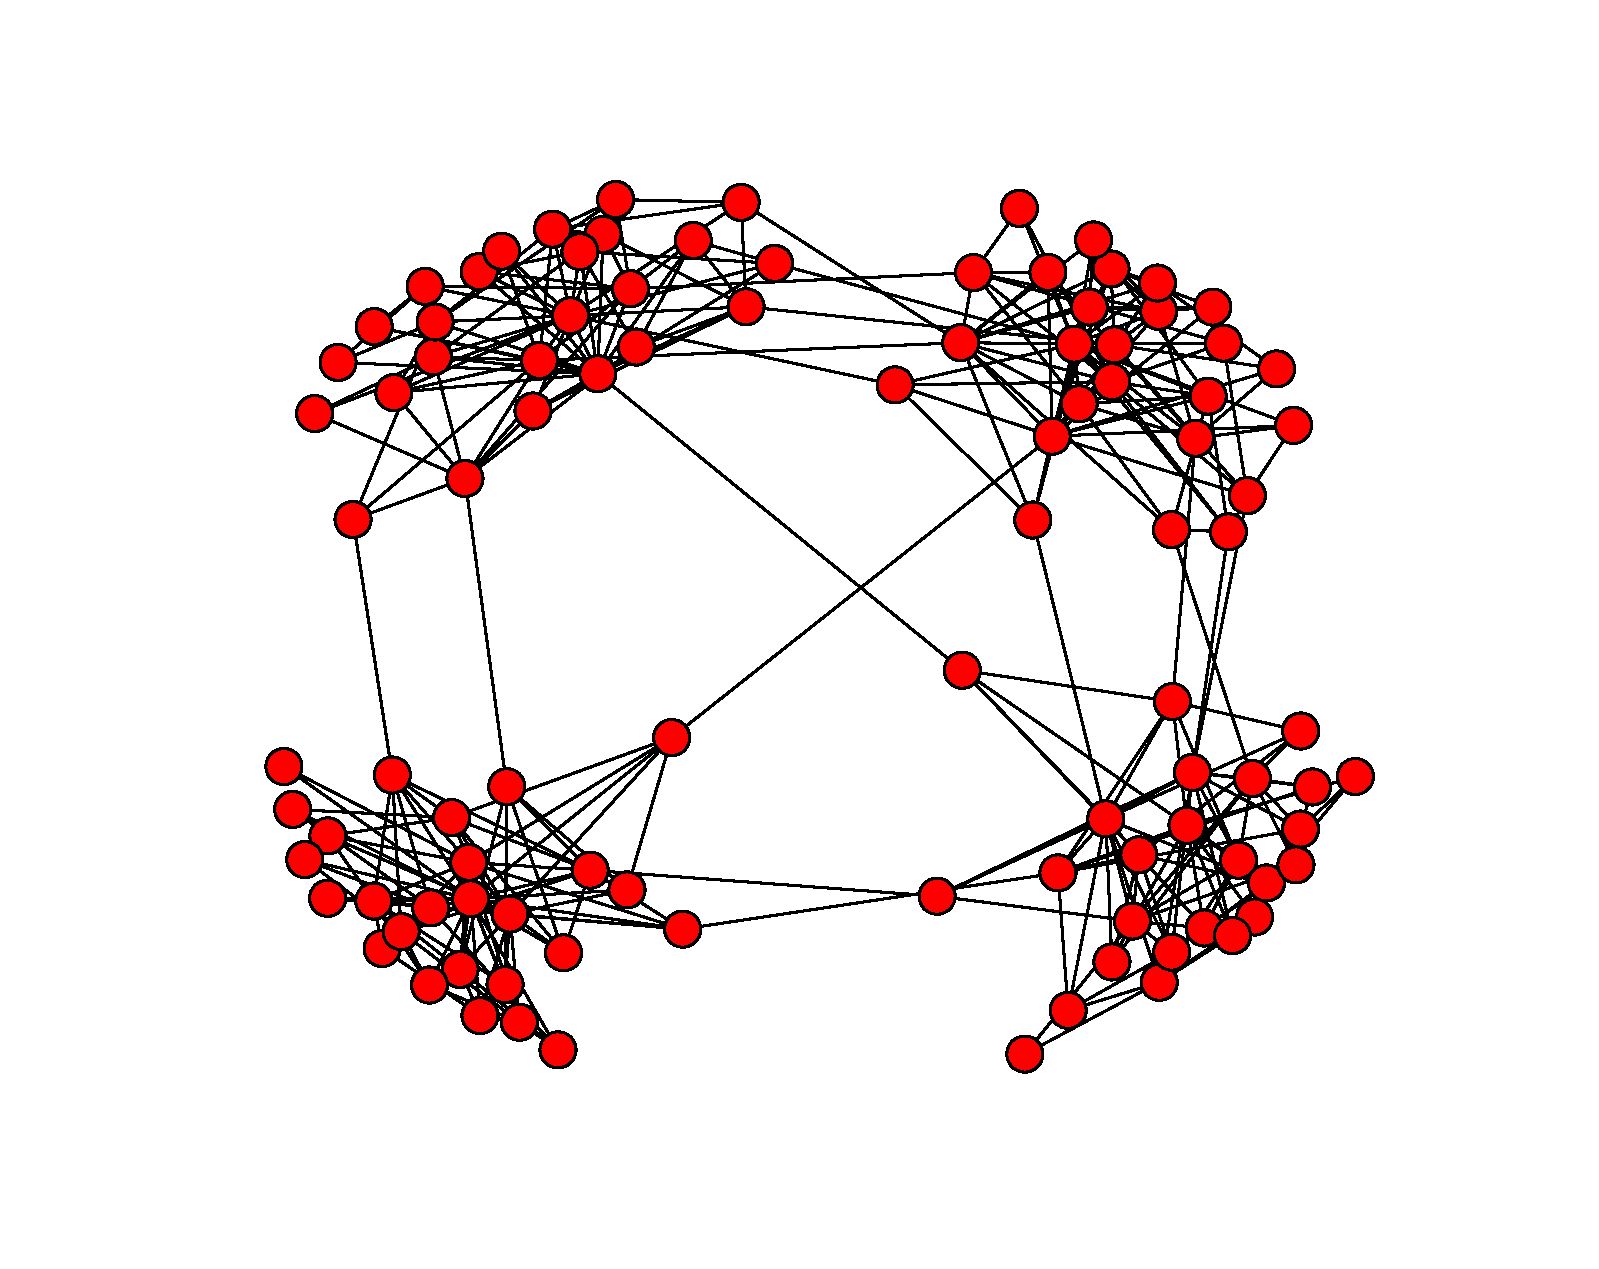
\includegraphics[scale=0.4]{images/topology/hierarchical_graph_4_dot05.pdf}
\caption{Hierarchical graph with $N=101$, $C=4$, $K=4$ and $\beta = 0.05$}
\label{fig:hierarchical graph 4}
\end{figure}

An example of a hierarchical graph can be seen in Figure \ref{fig:hierarchical graph 4} where $101$ initial agents are first divided into $4$ communities and then each edge is rewired with $\beta=0.05$ probability. 
The 4 communities are clearly visible and each community is loosely linked to each other maintaining low the short average path.

Same observation can be made by looking at the adjacency matrix of different hierarchical graphs.
Examples for hierarchical graphs with $C$ in $\{2,3,4\}$ for $\beta=0.1$ are visible in Figure  \ref{fig:hierarchical adjacency graph 0.1}, while for the same number of communities but with higher rewiring parameter $\beta=0.25$ can be seen in Figure \ref{fig:hierarchical adjacency graph 0.25}.

\begin{figure}[h]
        \centering
        \begin{subfigure}[b]{0.3\textwidth}
        	\centering
                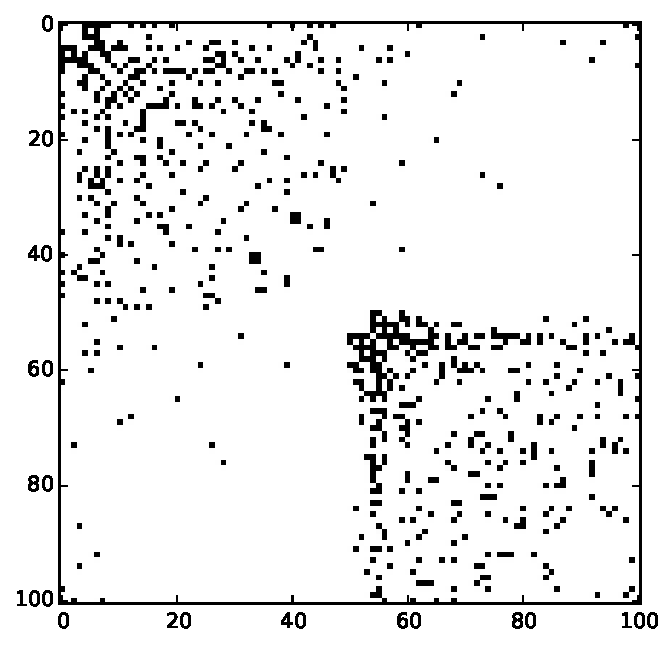
\includegraphics[width=\textwidth]{images/topology/hierarchical_adjacency_2_dot1.pdf}
                \caption{$C=2$}
        \end{subfigure}
        \begin{subfigure}[b]{0.3\textwidth}
        	\centering
                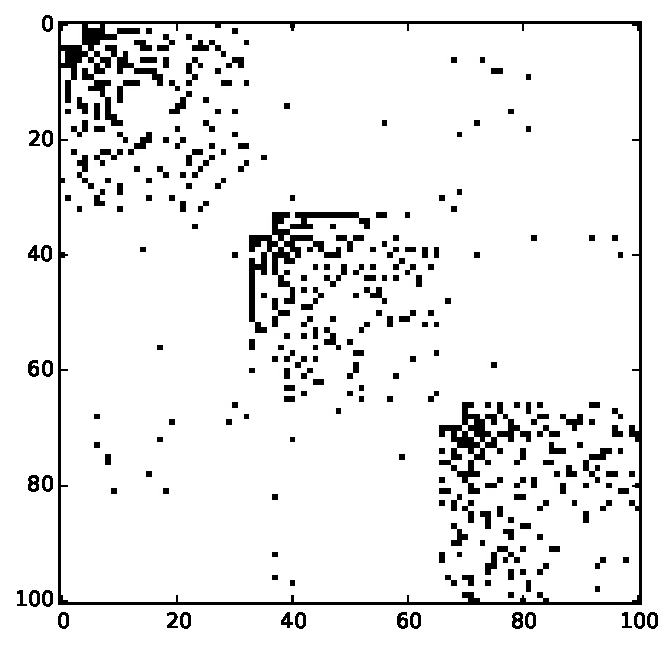
\includegraphics[width=\textwidth]{images/topology/hierarchical_adjacency_3_dot1.pdf}
                \caption{$C=3$}
        \end{subfigure}
        \begin{subfigure}[b]{0.3\textwidth}
        	\centering
                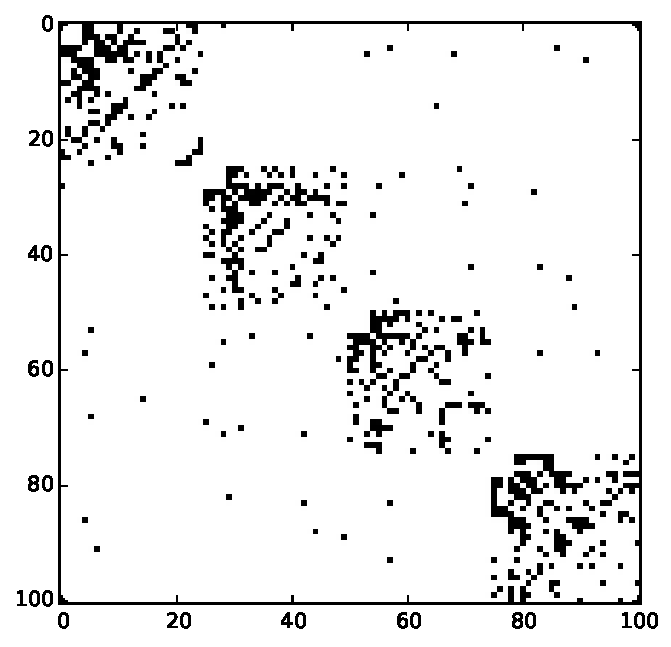
\includegraphics[width=\textwidth]{images/topology/hierarchical_adjacency_4_dot1.pdf}
                \caption{$C=4$}
        \end{subfigure}
        \caption{Hierarchical graph adjacency matrices with $N=101$, $K=5$ and $\beta =0.1$}
        \label{fig:hierarchical adjacency graph 0.1}
\end{figure}


\begin{figure}[h]
        \centering
        \begin{subfigure}[b]{0.3\textwidth}
        	\centering
                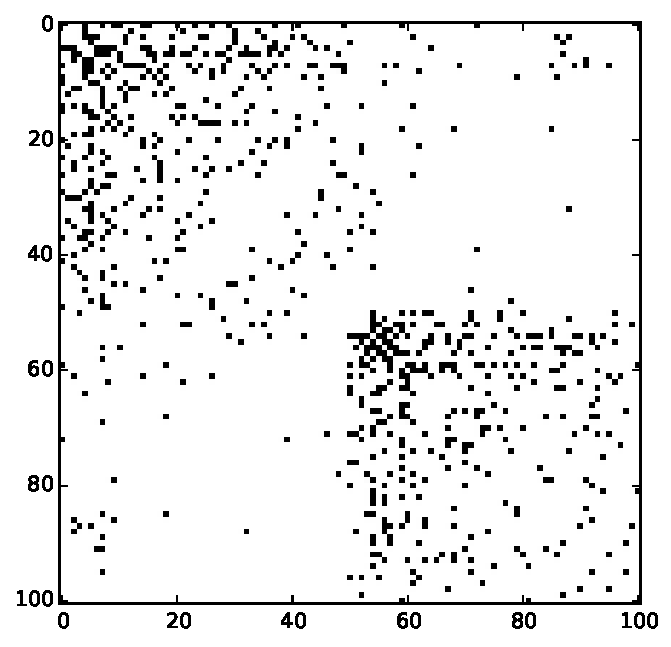
\includegraphics[width=\textwidth]{images/topology/hierarchical_adjacency_2_dot25.pdf}
                \caption{$C=2$}
        \end{subfigure}
        \begin{subfigure}[b]{0.3\textwidth}
        	\centering
                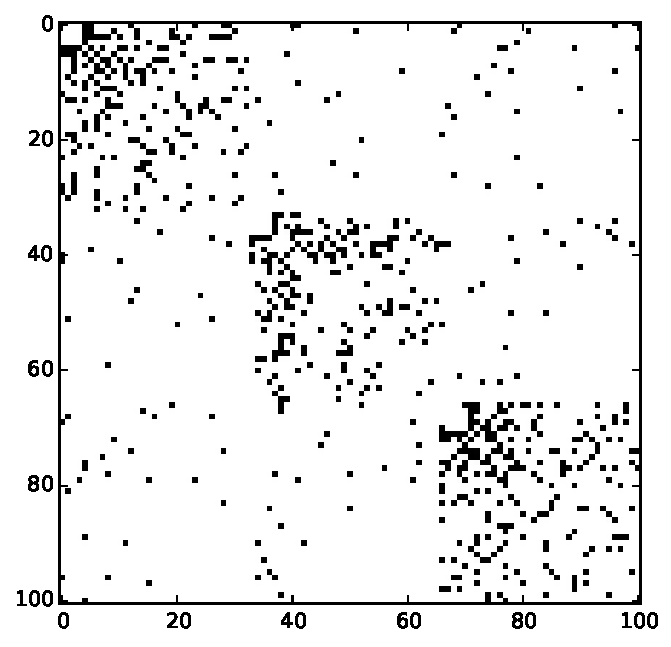
\includegraphics[width=\textwidth]{images/topology/hierarchical_adjacency_3_dot25.pdf}
                \caption{$C=3$}
        \end{subfigure}
        \begin{subfigure}[b]{0.3\textwidth}
        	\centering
                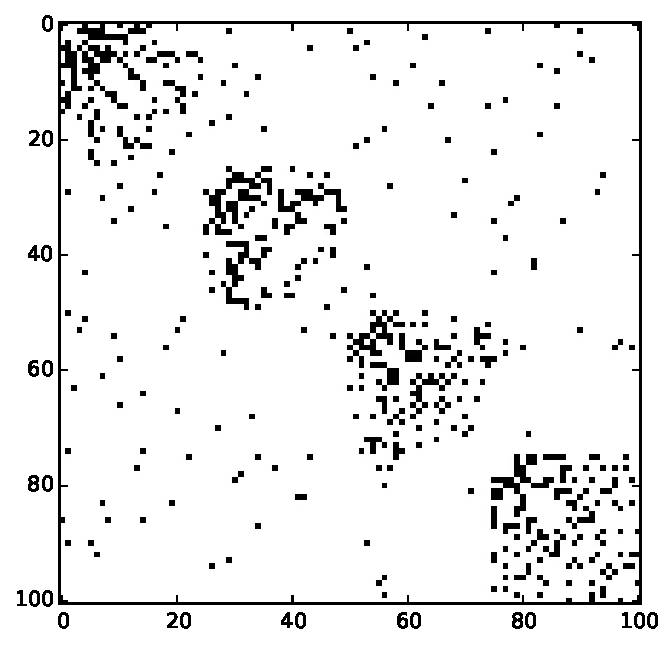
\includegraphics[width=\textwidth]{images/topology/hierarchical_adjacency_4_dot25.pdf}
                \caption{$C=4$}
        \end{subfigure}
        \caption{Hierarchical graph adjacency matrices with $N=101$, $K=5$ and $\beta =0.25$}
        \label{fig:hierarchical adjacency graph 0.25}
\end{figure}

We do not expect better or worse performance by using this structure for the vicinity in minority games, but the fact they are closely representative of real world network structures, we believe they need to be studied and analysed in order to find the best conditions under which these competitive systems perform.

\subsection{The algorithm}
\label{subsec:algorithm}

\section{Real world applications}
\label{sec:real world}

\subsection{Financial markets}
\label{subsec:financial markets}

\subsection{Delay Tolerant Networks}
\label{subsec:dtn}

\subsection{Smart energy resource allocation}
\label{subsec:smart energy}

\subsection{Computer resource allocation}
\label{subsec:computer resource}